\chapter[Neutral MSSM Higgs Search...]{The Search for neutral MSSM Higgs Bosons in the final state:
$\tau^{+}\tau^{-} \rightarrow e \mu + 4\nu$}

This chapter contain the main work of this thesis, reports about the search 
the neutral MSSM Higgs bonon decaying in tau pairs
and fully leptonic final state. This search is based on 2012 8 TeV data
recorded by ATLAS experiment at Large Hadron Collider.

Discovering the mechanism responsible for electroweak
symmetry-breaking and the origin of mass for elementary particles has been
one of the major goals of the physics program at the Large Hadron
Collider~(LHC)~\cite{LHC}.  In the Standard Model (SM) this mechanism
requires the existence of a single scalar particle, the Higgs
boson~\cite{ENGLERT,HIGGS,HIGGS2,HIGGS3,Guralnik:1964eu}.
In the Minimal Supersymmetric extension of the Standard Model
(MSSM)~\cite{MSSM1, MSSM2} the Higgs sector is composed of two Higgs
doublets of opposite hyper-charge, resulting in five observable Higgs
bosons.  Two of these Higgs bosons are neutral and $CP$-even
($h$,$H$), one is neutral and $CP$-odd ($A$) and two are charged
($H^\pm$).  At tree level their properties such as masses, widths and
branching ratios can be predicted in terms of only two parameters,
often chosen to be the mass of the $CP$-odd Higgs boson $m_A$, and
the ratio of the vacuum expectation values of the two Higgs doublets
$\tan\beta$ (more detail in chapter~\ref{}).  

This chapter is divided in three sections:
in section~\ref{sec:strategy} an introduction to experimental searches and to the strategy
of this particular analysis is given, in section~\ref{sec:bkg} is described the core of this thesis
work, i.e. the detail of the background modeling for this analysis, while in section~\ref{sec:result}
the result of the sarch are presented.


\clearpage

%\section{Inside Neutral MSSM Higgs}
%\section{What is a Search?}
%\section{Search First Principle}
%\section{Search Elements}
%\section{The Search in a Nutshel}
\section{The Search Strategy}
\label{sec:strategy}

\subsection{Motivation}

\begin{figure}[tp]
     \begin{center}

            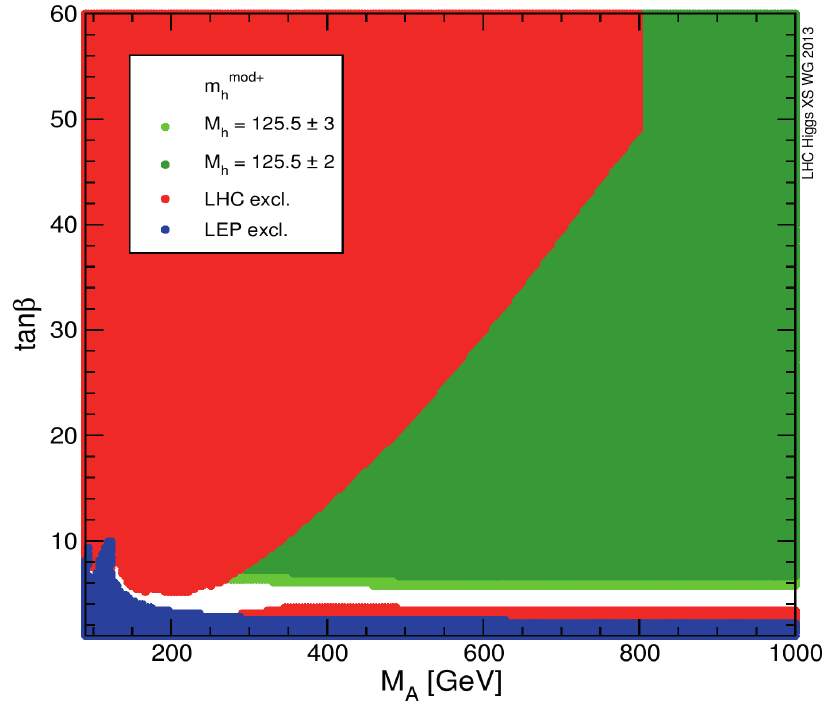
\includegraphics[width=0.5\textwidth]{figure/mh_mod.png}

    \end{center}
    \caption{$m_{A} - \text{tan}\beta$ plane for the  $m_{h}^{mod+}$ scenario, with excluded region
	from direct Higgs searches at Lep (blue) and LHC (red). The two green shades corresponds to
	the allowed parameter space for the assumption of $M_{h} = 125.5 \pm 2 (3)$ GeV. For more detail 
	see~\cite{}.}
   \label{fig:mhmod}
\end{figure}

Under the light of the recent discovery of a Higgs 
boson with mass of 125 GeV \cite{}, remains an open question
wheter this new particle constitute all the pieces of the Higgs
sector or if it is only one of several bosons predicted in some theories 
that go beyond the SM. The most recent measurements \cite{} of its
properties shows it to be, within experimental uncertainties, perfectly 
compatible with the SM Higgs boson, however such a new particle can 
be accomodated within several beyond the 
standard model (BSM) theories, this is particularly true for Super Symmetry. 

There are two approach to explore the Higgs sector:
studying the cupling of the Higgs boson with vector
bosons and fermions, given the unitarity property of scattering
aplitudes for longitudinal vectors and fermions, one can understand 
if this particle is  fully responsible for
the generation of the masses of all the other SM particles. 
Another approach is to directly search for %model dependent
for additional Higgses in a well defined model. In this thesis the last approach is 
followed, new particle are sought within the MSSM scenario (see chapter \ref{}). 

In the MSSM a Higgs boson with properties that  
resembles the one for a SM Higgs boson occures naturally in large regions 
of parameter space, for practical reason however,
% a point in the MSSM parameter space must now not only pass all the 
%experimental bounds on superparticle masses, but also lead to the prediction of a scalar with
%mass, production cross section and decay rates compatible with those measured at the LHC.
%it is not convenient to scan over a large parameter space as the MSSM has, for practical reason
is usefull to fix  parameter of the model to achieve what is called a benchmark
scenario. With the recenty discovery, bechmark scenario of the MSSM have been updated to fit
with the new constraints (more details on benchmark scenarios are in chapter~\ref{}), 
as an example in figure~\ref{} are reported the current exclusion limits
for one of those updated scenarios, $m_{h}^{mod+}$, the green area represents what is currently 
allowed in the $m_{A} - \text{tan}\beta$ plane showing that there is still plenty of room for BSM
Higges.

\subsection{How to search for new phenomena?} 
%\subsection{What is a search?} 
Typically new physics searches are looking for a signal 
that is additive on top of the background, an observation of an excess or exclusion of a signal
is then characterize by statistical statemetnts.  A \emph{statistical test}
is a rule used to reject or accept an hypotesis. An hypotesis is a statement about the distribution of the data.
In the search for new phenomena at the LHC frequentistic statistical tests are used~\cite{LHCstat},
where two hypotesis are compared:  the background only hypotesis $H_{0}$,
which plays the role of the null hypotesis, and the signal plus background hypotesis $H_{1}$, which is the alternative.
In this section an itroduction to LHC statistical procedure is given, for more details see section~\ref{sec:stat}.

In a search for new physics usually a \emph{signal region} is defined in data where 
events are counted,  the number of observed events $N_{SR}$ is a random
variable described by a Poisson distribution, in case the null hypotesis is true $\nu_{B}$ events are expected, while   
$\nu_{B} + \nu_{S}$ are expected for the $H_{1}$ alternative hyspotesis, 
the probability model for null and the alternate hypotesis is ithen respectively 
$\text{Pois}(N_{SR}|\nu_{B})$ and $\text{Pois}(N_{SR}|\nu_{B} + \nu_{S})$.
The evidence for a signal shows up as an excess of 
events, a way to quantify the conpatibility of the null hypotesis with data
is to make a \emph{significance} test, this leads to the calculation of the probability that 
the background-only would produce at least as many
as the observed events, this is the so called of p-value, which in this case is expressed by the formula:
$$
\text{p-value} = \sum_{n=N_{SR}}^{\infty} \text{Pois}(n|\nu_{B})
$$
Calculating  p-value is a way to characterize an excess, in high energy physics the commonly accepted p-value that 
qualifies as discovery is $2.87 \times 10^{-7}$, which translated to the probability of a gaussian 
distribution correspond to five standard deviation. 

In case no excess is observed, the procedure is to build a statisctical test where the 
null hypotesis is accepted and at the same time the signal hypotesis
is rejected with a fixed predetermined probability, called confidence level.
A statistical test is a rule that defines a region in the space of data for which
a given hypotesis can be accepted or rejected, often rather than using a full set 
of data $\mathcal{D}$, it is convenient to define a \emph{test statistic}, T, which is usually a single
number computed from the data, the two hypotesis implies different distributions for T, 
then one defines an acceptance region \emph{W} in terms of the test statistic, if 
$T \in W$ the $H_{0}$ is rejected and $H_{1}$ accepted and vice versa,
the probability with which one rejects $H_{1}$ or $H_{0}$ is then given by the choice of
\emph{W} and T. Neuman and Person provided a framework for hypotesis testing that addresses the 
choice of the test statistic \cite{NP}.
%such that 
%$P(T \in W | H_{0}) \leq \alpha$, where $\apha$ is the size of the test and correspond to the probability
%for which $H_{0}$ is rejected when is true, 

A discriminating variable is often used to help separating signal and backgrounds, this can be any of the observables of
the experiment, a usually chosen observable is for example the invariant mass of final state particles, 
knowing the probability density function $f(x)$ for this observable for the two hypotesis one can complete the above
mentioned statistical model with what is called a marked Poisson for a set of data $\mathcal{D}$:
$$
\text{Pois}(N_{SR}|\nu) \prod_{i \in \mathcal{D}}^{N_{SR}} f(x_{i} | \vec{\theta})
$$
here is made explicit that $f(x)$ depends also on a set of additional parameter $\vec{\theta}$, called nuissance
parameter, those embed effects like detector mismodeling or theoretical uncertainty.
With the use of a discriminating variable one can take advantage of additional information  
to disentangle between signal and backgrounds.

%A statistical test is a rule that define a region in parameter space for which  a given hypotesis can be accepted or rejected.
%Often rather than using a full set of data $\vec{X}$, it is convenient to define a \emph{test statistic}, t, which is usually a single
%number, it is a quantity calculated out of the data, a mapping of a set of measurements into a single number. The test statistic, that is usually
%connected to the discriminating variable, would then have a different distribution for the different hypotesis, one can then define $\alpha$
%called the size of the test and $t_{\alpha}$ for which $P(t < t_{\alpha} | H_{0}) \leq \alpha$ then in this case $H_{0}$ is rejected.

%- Alternative: NP provided a framework for hypotesis testing that addresses the choice of the test statistic. First one defines 
%an acceptance region in terms of a test statistic, such that if $T(\vec{X}) < t_{\alpha}$ one accepts the null hypotesis. 
%One can think of $T(\vec{X}) = t_{\alpha}$ as a counturn in the space of the data which is the boundary to this acceptance region.
%Then one defines the size of the test $\alpha$ which is the probability for the null hypotesis to be rejected when true,
%the test is totally asymmetric: if the null hypotesis is rejected then the alternate is accepted (is this true??)....

Summarizing, there are several ingredients that constitute a search for new physics and will be discussed 
with more details in the following sections:
\begin{itemize}
	\item Define a signal region in data where signal is enhanced with respect to the backgrounds, detailed in section \ref{bla}
	\item Define a discriminating variable which is usefull to disentangle between signal and backgrounds, section \ref{bla}
	\item Define the probability model, i.e., the expectation for the distribution of the discriminating variable
		 for signal and background hypotesis, this is one of the most importat
		point of a search and main part of the work of this thesis, detailed in section \ref{bla}
	\item Define a test statistics, which is detailed for the LHC in section \ref{bla}.
\end{itemize}

%
%-----------------------------------------------------------
%
%
%The language of searching for new phenomena is statistics, the aim of a search is to exclude certain region of parameter space for a 
%defined model or (this is quantified by) observe an excess... Statistical methods define procedure for characterising  
%an observation of excess or exclusion of a signal.
%Frequentist hypotesis test provide a rule for accepting or rejecting hypotesis depending on the outcome of a measurement.
%
%To compare the compatibility of the data with the background-only and signal+background hypoteses a so called test statistic is constructed.
%
%An Hypotesis is a statement about the distribution of the data, a \emph{statistical test} is a rule used to reject or accept an hypotesis.
%This is done defining a parameter space, a region 
%
%We use the Neyman-person hypotesis test to set exclusion limits, to characterize instead the significance of an observation we use the p-value.
%With some test statistics one can set a region with fixed probability for the signal to occurr, one can then accept-reject this hypotesis with
%fixed probability, the test is symmetric: rejecting $H_{0}$ means accept $H_{1}$.
%
%Si ma si parla sempre di numero di eventi.... Fare esempio concreto!
%
%Frequentist hypo test ---> 2 hypo necessary
%*) search e' una cifra di cose, nella stostra accezione una search significa looking for excess of events with a particular topology.
%The language of a search is statistics so we are going to define some quantities:
%*) Test of hypotesys: define a test to say if this hypo is true
%*) calculate the probability, under the hypo, to observe a deviation at least as big as the one observed in data, this is the definition of p-value.
%This is usefull in case you do have a signal, what about if not?
%*) you define an additional hypotesis, signal hypo, and ten you can exclude a certain range of parameter space with a pre-fixed probability.
%*) Il tutto si riduce a contare eventi nella signal region. Next sections define how we built this signal region and why.


\begin{figure}[tp]
     \begin{center}

            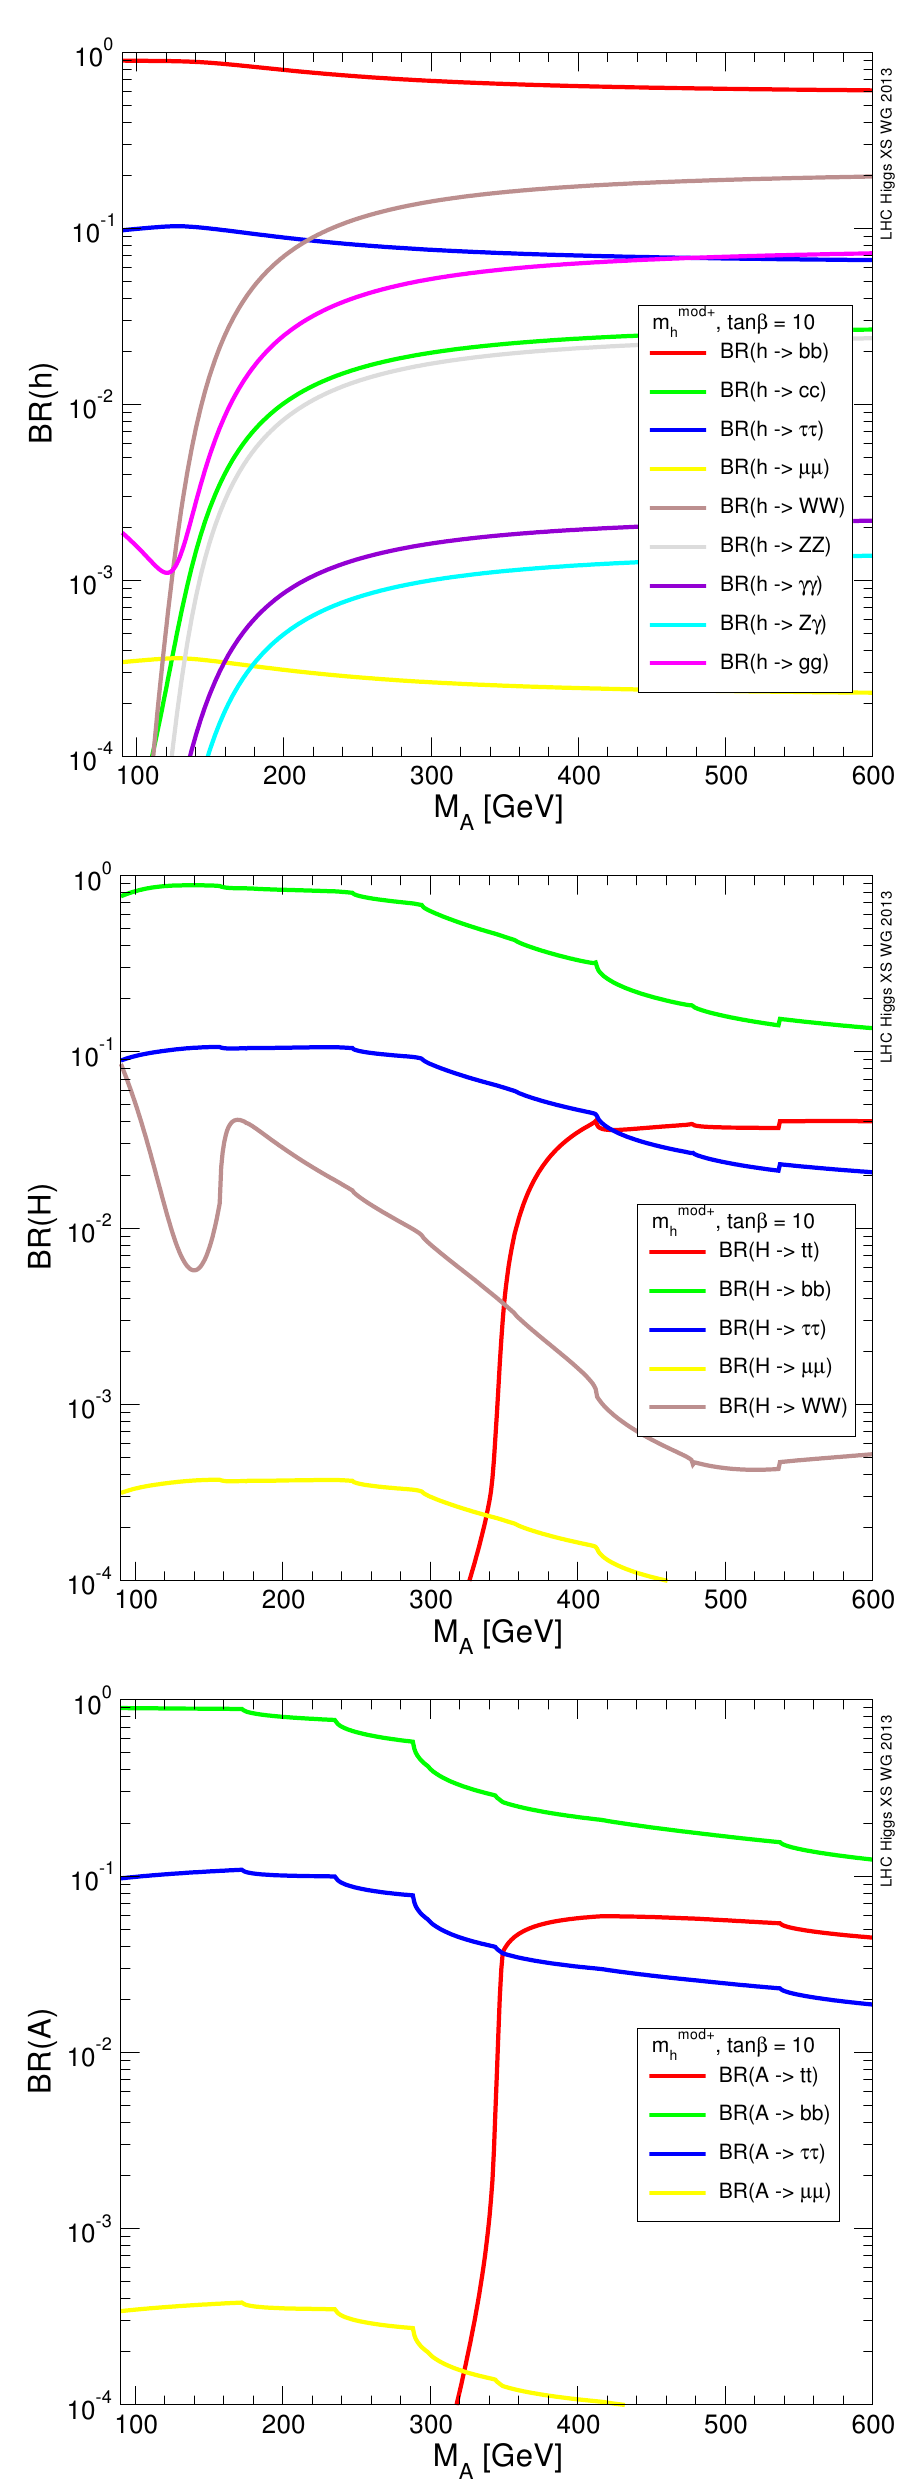
\includegraphics[width=0.5\textwidth]{figure/br.png}

    \end{center}
    \caption{Branching fraction for the MSSM neutral higgses in the bla scenario.}
   \label{fig:br}

\end{figure}

\begin{figure}[tp]
     \begin{center}

            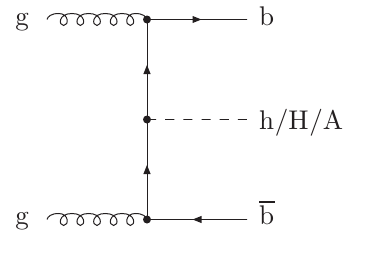
\includegraphics[width=0.45\textwidth]{figure/bba.png}
            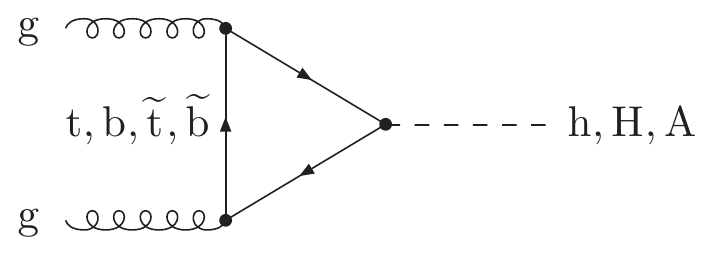
\includegraphics[width=0.45\textwidth]{figure/ggf.png}

    \end{center}
    \caption{Diagram for b-associated production and gluon-gluon fusion for MSSM neutral Higgs.}
   \label{fig:prod}
\end{figure}

\begin{figure}[tp]
     \begin{center}

            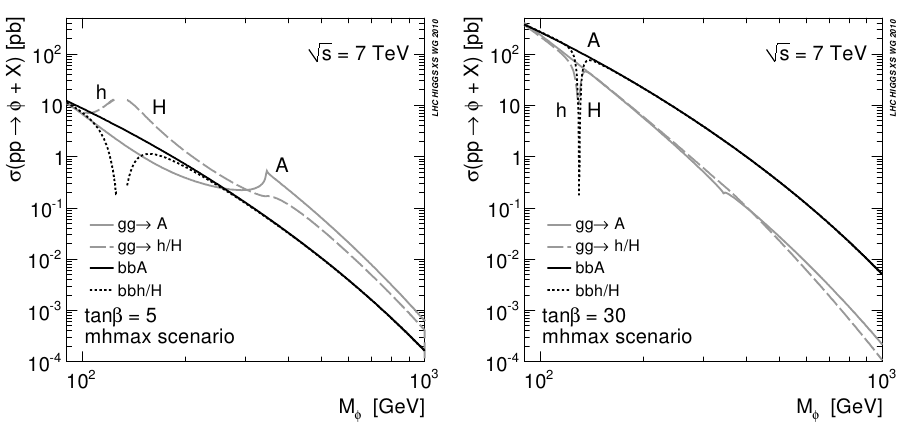
\includegraphics[width=0.5\textwidth]{figure/xsec.png}

    \end{center}
    \caption{Cross section for different MSSM neutral Higgs production mode.}
   \label{fig:xsec}
\end{figure}

\subsection{Signal Topology}
This section describes the strategy to enhance the search sensitivity 
taking advantage of the signal topology.
The Sensitivity of a search is the signal strenght that is expected to be  excluded 
in case of no signal. If one is searching for a rare process, then the analysis strategy, i.e. the
plan or the steps to enhance the signal sensitivity of the search, is crucial.
A further consideration is that this search is complementary to the Standard Model
Higgs search in tau final state, the focus is then on non explored phase space from SM.

In the MSSM for large region of parameter space one found that one of the 
$CP$-even neutral Higgses is has properties that resemble the one of the SM Higgs,
this is usually the case for the lightest Higgs, \emph{h}, the other two, $H$ and $A$, 
thend to be degenerate in mass and decouple from gauge bosons.
An interesting fenomenological point is that the coupling of the latter
two Higgses with down (up) type fermions are enhanced
(suppressed) by $\tan\beta$, meaning that for large $\tan\beta$
bottom-quark and $\tau$ lepton will play a more important role than in
the SM case either for production and decay.

The production of the neutral $CP$-even MSSM Higgs bosons at hadron
colliders proceeds via the same processes as for the SM Higgs
production. However, the pseudoscalar $A$ instead cannot be produced
in association with gauge bosons or in vector boson fusion (VBF) at
tree-level, as this coupling is forbidden due to $CP$-invariance.  At
the LHC one of the most relevant production mechanisms for the MSSM
Higgs bosons is gluon-gluon fusion, $gg\rightarrow A/H/h$. In
addition, the production in association with $b$-quarks becomes
important for large value of $\tan\beta$. Those are the two production mechanism
that are considered in this analysis, figure~\ref{} shows the feyinman-diagram
for those processes. The search is divided in two category which are optimized
for the two different production mode considered, in the gluon-fusion category
is requred a b-jet veto, in fact no b-jet in the final state are present for this
production mode. In contrast a a b-jet tag is required for b-associated production,
this category is expected to be very sensitive to $\tan\beta$. The two category are
ortogonal and present different backgrounds contributions, which can be
optimized separately. 

The decays of the neutral
MSSM Higgs bosons (in the assumption that all supersymmetric particle
are heavy enough) are the same as for the SM one with the already
cited exception of $A$. Figure~\ref{} shows the decay branching fractions
for $H$ and $A$, as a function of the mass and for $\tan\beta = $, 
the decay into tau pair is the most important after $b\bar{b}$. The 
decay channel in $b\bar{b}$ is challenging due to the huge background from
QCD multi-jet, in this analysis the decay in tau pairs is choosen.
In this thesis only cases in which the taus decay one in $e + 2\nu$ and
the other in $\mu + 2\nu$ are considered, This final state corresponds to a total
$\tau^+\tau^-$ branching ratio of approximately 6\%.
 
%Searches for neutral MSSM Higgs bosons have been performed at
%LEP~\cite{LEPLimits}, the
%Tevatron~\cite{TevatronLimits1,TevatronLimits2,TevatronLimits3,TevatronLimits4,TevatronLimits5,TevatronLimits6}
%and the LHC~\cite{CMSLimit, ATLASLimit}.  In this note a search for
%neutral MSSM Higgs bosons with the ATLAS experiment at CERN is
%presented, using proton-proton collisions at centre-of-mass energy of
%8~TeV, with a recorded integrated luminosity of
%$20.3 \ifb$.

Summarising, the signal topology is characterised by a final state with an
electron, a muon, and missing transverse energy due to the
presence of four neutrinos from the $\tau$ decays. Furthermore, the
final state may be split by the presence or
absence of a $b$-quark initiated jet, depending on the production
process. This signature is achieved experimentally by requiring:
an OR of a single elecron and an electron-muon trigger, exactly
one reconstructed electron and one muon in the final state, the two 
leptons should be of opposite charge and isolated. With isolation                               %
it's meant that in a cone around the lepton there should be little energy deposit (should not be sorraunded by                 
other particle, common of non-promt leptons coming from jets). More detail about isolation properties
are detailed in section ~\ref{sec:bkg}. Full detail on actual preselections regarding all the quality requirements    
on object reconstruction are reported in appendix~\ref{ap:presel}.                                                             
   


\subsection{How to deal with Backgrounds}
%\subsection{Selections}
The signal topology described in the previous section common to many other processes, unfortunately 
those have higher cross section than the signal we are looking for,
%magari qui si puo' dire che ci sono diversi metodi per aumentare S/B 
a set of additional selection has been studied to enhance the sensitivity of the search, or in other words,
to increase the signal  to background  ratio. The most important backgrounds to this search are the production of
 $\Ztautau $ + jets, the top quark ($t\bar{t}$ and single top production is intended), diboson production 
(like $WW$ or $ZZ$ events) and events with non-prompt leptons coming from QCD multi-jet (in short QCD multi-jet).
Vector bosons production like  $\Wlnu$ or $\Zll$ + jets (with l here meanung either $e$ or $\mu$) are also considered,
however those processes have a limited impact.

The final state of Higgs decaying into tau pair coincide with the one from  $\Ztautau$  process, this is then an irreducible 
background, however exploiting the different kinematics of the Higgs decay and the other backgrounds it possible to distinguish 
between signal and them.
%do present different kinematics  and is possible to exploit 
%Exploiting the kinematics of the Higgs deacaying
The most stiking is that the higgs (like $\Ztautau$) selecting an electron and one muon
coming from the tau decay, due to the high mass the taus will be back to back and their decay products will be highly boosted,
this gives rise to two feature: the mu-e will be more likely back to back, as you can see in figure~\ref{fig:selections} that shows the angle between the
leptons in the transverse plane 
$\Delta\phi = |\phi_{e} - \phi_{\mu}| $\footnote{This is actually more complicated: one has to take care of the sign of $\phi$ see chapter\ref{c:detector}}
prefer configuration in wich the leptons are in opposite emisphere.
Furthermore the neutrinos will be more likely collinear with the leptons (given the high boost the taus recive from Higgs decay).
This feature can be matematically seen as the sum of scalar product between missing energy and the leptons four-vectors in the
transverse plane, if the vectors are normalised to unit versors then what remains is a relation only between angles:
$$ \hat{E}_{T}^{miss} \cdot ( \hat{P}_{T}^{\mu} + \hat{P}_{T}^{e} ) = cos(\Delta\phi_{E_{T},\mu}) + cos(\Delta\phi_{E_{T},e})  $$
In the assuption of collinearity and of leptons back-to-back that scalar product  is equal to zero, in fact  it would be equal 
to zero for each of the  neutrinos being it collinear with one lepton and back-to-back with the other.
As can be seen from figure~\ref{fig:selections} in fact the distribution of that variable 
has its more likely values at zero. These two feature can be used to distinguish between mu-e coming from decay from highly 
boosted object and the one coming from W decays in top or in dibosons backgrounds which will have a more spread distribution.
In b-veto category these two selections are sufficient to suppress contribution from dibosons,
no other selection is applied in this category because it has been shown to not bring significant improvement.

In the b-tag category the situation is different, 
the  request of b-jet enhance backgrounds with high jet activity as top production, given the relatively low
jet activity of our Higgs events (also in the case of b-associated production) it's possible to separate them from
top production which instead is very likely to have 2 or more highly enegetic jets in the event, requesting a small jet activity, 
this is achieved by requesting the sum of the jets transverse momentum to be small, we call this variable $\Ht$.
Another feature that distinguish top pair production from Higgs is the much higher invariant mass of the former final state,
in the transverse plane all the leptons will tend to have a higher momentum, we then use the sum of lepton \pt and \met as
a discriminating variable, requesting it to be small. Figure~\ref{} shows the distribution of these two variables 
after the request of a b-jet.

Plots with MMC mass as a function of selection that shows how effective they are in reducing backgrounds.

In table~\ref{} a summary of all the selection variable used with their optimized cut values is reported.
While in table~\ref{} the number of events that survises at each cut stage for different background is reported.

\begin{figure}[htp]
     \begin{center}

            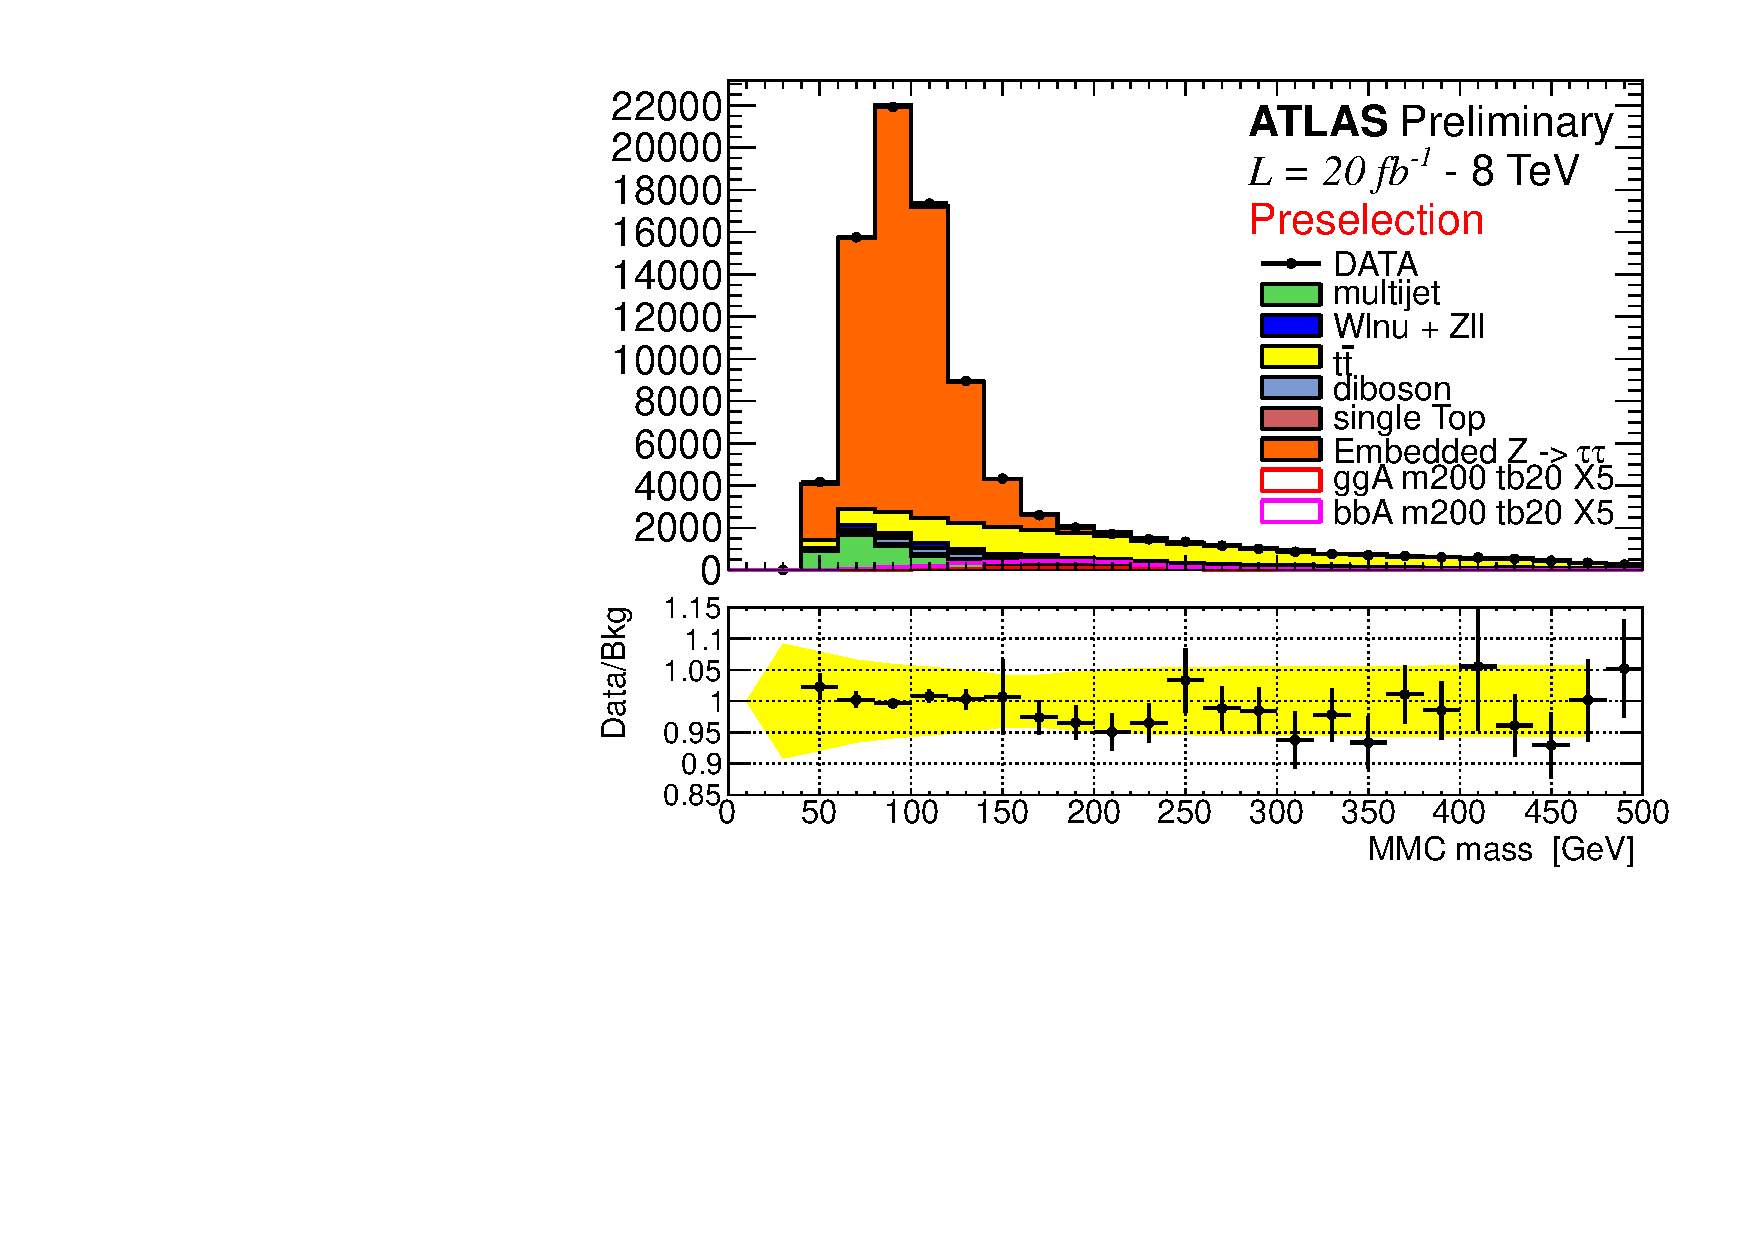
\includegraphics[page=1,width=0.45\textwidth]{figure/std_plots_presel.pdf}
            \includegraphics[page=2,width=0.45\textwidth]{figure/std_plots_presel.pdf}
            \includegraphics[page=3,width=0.45\textwidth]{figure/std_plots_presel.pdf}
            \includegraphics[page=4,width=0.45\textwidth]{figure/std_plots_presel.pdf}
            \includegraphics[page=5,width=0.45\textwidth]{figure/std_plots_presel.pdf}

    \end{center}
    \caption{bla}
   \label{fig:selections}
\end{figure}


\subsection{Missing Mass Calculator}

% si potrebbe anche aggiungere un pezzo di statistica parlando di pdf fatta da histo....
 
Accurate invariant mass reconstruction of a di-tau system is a challenging task due to the escaping neutrinos.
In this analysis, with four neutrinos in the final state, the number of unknown largely exceed the number of constraints,
several approximation are possible to further constraint the neutrinos, for example assuming them collinear to the 
other leptons from tau decay, however those approximation suffers of limitations. 

In this analysis we use the so called missing mass calculator (MMC)~\cite{MMC}
technique for the calculation of the di-tau system invariant mass. This technique employs additional 
information from the well known tau decay to constraint the system, this is achieved by minimising a likelihood function 
defined in the kinematically allowed phase space region, the result is a more precise measurement of the di-tau 
system invariant mass and a considerable improvement in resolution. The invariant mass distribution 
calculated with the MMC technique is referred in the following as $\mmc$ and is used as discriminating 
variable in the limits setting.



